\section{Overview}

In this chapter I explore the use of unsupervised word embeddings to aid the
task of Spanish \vsd. The work on English \vsd~done in Chapter
\ref{chapter:supervised} served as a comparison point to the work done for
Spanish, however to simplify the study of semi-supervised techniques I am from
now focusing on Spanish only.

The previous chapter showed us two of the main problems with the purely
supervised approaches with small labeled data: overfit of the data and little
coverage. The model learns to adapt to the available features, and although it
manages to do so well, it generalizes poorly, thus ends up overfitting. The
coverage of the data, on the other hand, depends on the amount of labeled data
available, which was established to be small. 

The previous chapter also showed that the size of the training dataset affects
the final performance of a model. Based on these results it is possible to
argue that the reason behind this phenomenon is that the more data there is,
the more features can be included in the model. Thus, new examples have better
representation because those features which represent them are more probably
included in the training dataset already.

To tackle this coverage problem, I want to expand the labeled data with new
data from unlabeled sources while keeping the effort of human annotation to a
minimum. However, in order to do so, I first need to find a way for the
available data to decrease the tendency to overfit, as I need a model to
generalize well to new examples so these add to the coverage of the model. I
will explore the impact of adding more examples with low annotation cost in the
following chapter. In this chapter I will focus on reducing the tendency to
overfit of classic supervised approaches.

Hand-crafted features pose a problem for generalization because they are are
literally taken from the labeled dataset, and thus do not play well with domain
change. This is important because the labeled data is contained in one
particular domain, the journalistic domain, because it is taken from a
newspaper. However, the model should adapt to other domains as well.

Finally, there are two other latent problems of the hand-crafted features
representations described in the previous Chapter, which add to the complexity
of any problem one would like to represent: high dimensionality and sparseness
of the representations. The dimensionality, as we saw in Section
\ref{sec:supervised:features} can be managed through some dimensionality
reduction technique (i.e. the {\em hashing trick}). Nonetheless, the sparseness
is still a problem, as most of the designed features occur on a single instance
basis, thus the representation vectors have little information. This high
dimensionality and sparseness of the data adds to the computational cost of
solving the problem with classifiers. 

To deal with these problems of sparse representations, I apply unsupervised
word representation methods, namely Word2Vec \cite{Mikolov2013}. These
techniques have recently gained attention in the natural language processing
community, specially with the resurgence of neural networks and deep learning.
These are called word embeddings and represent words with fewer dimensions and
dense vectors.

This chapter takes the domain and experiments from the previous chapter, i.e.
verb sense disambiguation for Spanish, and develops on new experiments upon
this basis, with the addition of word embeddings as features for the models.

This chapter will test the following hypothesis:

\begin{hypothesis}\label{hyp:embeddings}
  Unsupervised representations improve upon supervised models by avoiding the
  overfitting caused by the features taken from the same dataset where the
  model is trained. 
\end{hypothesis}

I will do this by proving the following subhypotheses:

\begin{subhypothesis}\label{hyp:embeddings:1}
  The performance of an unsupervised representation depends on the domain of
  the unlabeled dataset where they are trained. 
\end{subhypothesis}

\begin{subhypothesis}\label{hyp:embeddings:2}
  Using word embeddings produces less overfitting over supervised models than
  hand-crafted features.
\end{subhypothesis}

These hypotheses will be tested using the following layout:

\begin{itemize}
  \item Experiment \ref{exp:embeddings:1} reports the performance of
    different representations, which can be supervised or
    unsupervised. The performance is measured by the macro and weighted
    average F1-score (Metric \ref{met:1}). Results shown in
    Section \ref{sec:embeddings:hyp:1} serve to accept Hypothesis
    \ref{hyp:supervised:1}, that the domain where word embeddings are obtained
    affects the final performance of the model.
  \item Experiment \ref{exp:embeddings:2} reports the variance of different
    models trained over different subsets of the training data. This variance
    is measured by Metric \ref{met:3} which reflects the tendency of a model to
    overfit, with aid of the learning curve. From this experiment and metric,
    using different visualizations according to the task, I show that the
    classifier is less prone to overfitting using word embeddings instead of
    hand-crafted features as stated by Hypothesis
    \ref{hyp:embeddings:2}. 
\end{itemize}

In Section \ref{sec:embeddings:previous} I recapitulate on previous work
on unsupervised representations and word embeddings. The special
focus is on the algorithm of word2vec. I also point out the work
done in \wsd~done using word embeddings.

In Section \ref{sec:embeddings:methodology} I explain all relevant items
concerning what is used to carry out the experimentation of this chapter.
First, in Section \ref{sec:embeddings:resources} I introduce the resources
I work with. A quick recap of the SenSem corpus is done, followed by the
unlabeled corpora used to train the word embeddings: SBWCE, journalistic
corpora, and regulations corpora. In Section \ref{sec:embeddings:features} I
describe the two types of features used for experimentation: supervised
features from the previous chapter and word embeddings trained from the
unlabeled corpora. Section \ref{sec:embeddings:experiments} lists the
experiments. Section \ref{sec:embeddings:metrics} lists the set of metrics
I use to measure the experiments.

Section \ref{sec:embeddings:results} reports the results of the experiments and
analyzes them in order to accept or reject the stated hypotheses of the
chapter.

Finally Section \ref{sec:embeddings:conclusions} draws the conclusions of this
chapter, recapitulating the Hypotheses and the implications of accepting or
rejecting them according to the evidence gathered in the results. It states the
shortcomings of the methods explored in this chapter and what I want to
accomplish on the next. It ends by outlining future work.

\section{Relevant work}\label{sec:embeddings:previous}

The method I explored the most for this chapter is the one proposed by Mikolov
et al. \cite{Mikolov2013a}: the skip-gram model with negative sampling. It
consists of a language model which maximizes the probability of a pair of words
(i.e. a skip-gram) co-occurring in some natural language text, while minimizing
the probability of a pair of random words co-occurring. For more detail on this
process please refer to Chapter \ref{chapter:domain_background}, Section
\ref{sec:domain_background:embeddings}.

There are however other approximations to unsupervised word representations,
which are very well explored on the work by Turian et al.
\cite{Turian:2010:WRS:1858681.1858721}. In this work, the authors improve the
accuracy of different existing natural language processing systems by using
unsupervised word representations as features.

On \wsd~systems, as explained in Chapter \ref{chapter:domain_background},
Section \ref{sec:domain_background:embeddings}, Taghipour and Ng
\cite{Taghipour2015SemiSupervisedWS} show the use of word embeddings
consistently improve the accuracy of the SemEval lexical sample and all-words
tasks and also in a domain-specific lexical sample task. Rothe and Sch\"utze
\cite{rothe-schutze:2015:ACL-IJCNLP} presented a system to learn embeddings for
synsets/lexemes. Finally, there is a good work on word embeddings as features
for \wsd~by Iacobacci et al. \cite{iacobacci-pilehvar-navigli:2016:P16-1}.

For Spanish \wsd, to my knowledge, there is little to none work done. I was
only able to find my own on which this thesis expands upon
\cite{cardellinodisjoint}.

\section{Methodology}\label{sec:embeddings:methodology}

This chapter explores how word embeddings aid a supervised learning classifier
(e.g. multilayer perceptron) by replacing supervised hand-crafted features.
From this Chapter onwards, there is an important remark: the phrases {\em word
embeddings} and {\em word vectors} can be used interchangeably.

\subsection{Resources}\label{sec:embeddings:resources}

There are two kinds of resources needed for the experimentation done in this
chapter: the labeled corpora to train the supervised classifier, and the
unlabeled corpora to train the unsupervised representations (word embeddings).

In contrast to the previous Chapter, the experimentation is done only on the
Spanish data, as this is my main concern of study and the previous chapter
provided enough information from the English dataset to assert the validity of
the supervised models.

\subsubsection{SenSem}

SenSem serves as the main resource to train the \vsd~model as the labeled
data. It is described in detail in Section \ref{sec:supervised:sensem}. Please
refer the Section for more information.

\subsubsection{SBWCE}\label{sec:embeddings:sbwce}

The main resource from where the word embeddings used in the experiments of
this Chapter come from is the {\em Spanish Billion Words Corpus and Embeddings}
\cite{cardellinoSBWCE} (SBWCE), which is a compilation of more than 1.4 billion
raw words of the Spanish language, taken from different sources available on
Internet, most of them coming from corpora used for statistical machine
translation tasks, as well as corpora from the Wikimedia foundation, which
makes it a general domain corpus.

The corpus has over 45 million sentences with more than 3 million unique
tokens. Is also preprocessed to remove all the punctuation symbols and replace
all the digits with the tag ``\digito''.

\subsubsection{Journalistic Corpus}\label{sec:embeddings:journal}

SenSem provides an annotated corpus based on two newspapers from the region of
Catalunya in Spain: ``El Peri\'odico'' and ``La Vanguardia''. This make the
resource heavily based on senses which have more to do with the journalistic
domain. Thus, to check on Hypothesis \ref{hyp:embeddings:1} we needed to
train some unsupervised representations from a journalistic domain corpus.

I extracted the documents coming from journalistic sources available on the
SBWCE and other newspapers available online. In comparison to the SBWCE
corpus, the corpus we could gather for this task was much smaller, having
nearly 71 million words available, which became 70 million after filtering out
all those words with less than 3 occurrences. There was a final list of
approximately 240 thousand unique words to generate the word embeddings which
dimension was 50.

\subsubsection{Regulations Corpus}

Finally, to test Hypothesis \ref{hyp:embeddings:2} I also need a specific
domain corpus, but one that is not from the same domain the SenSem is based
upon. Originally I intended to use a corpus based on free software
documentation, as the technical aspect of such corpora would be a good contrast
to that of a journalistic domain corpora. However, the available corpus I could
find online was too small to generate good word embeddings representations.

Besides journalistic domain texts, the other domain available with enough
information available was a regulations corpora, based on corpora such as the
European Parliament, the United Nations, etc. where the text is more formal as
it deals with laws, normatives, etc.

The amount of data available is approximately the same available in the
Journalistic Corpus, with 72 million tokens, but a vocabulary of 100 thousand
unique words and embeddings of dimension 50.

\subsection{Features}\label{sec:embeddings:features}

\subsubsection{Supervised}

For the purely supervised experiments, the data is represented using all the
features described in Section \ref{sec:supervised:features} and the {\em
hashing trick} presented in Section \ref{sec:supervised:hashing}.

\subsubsection{Word embeddings}\label{sec:embeddings:embeddings}

For the word embeddings representations I used Word2Vec algorithm
\cite{Mikolov2013} to train the word embeddings from the unlabeled corpora.
The first set of word embeddings, for the general domain experiments, are the
pre-trained available on the SBWCE.

The word embeddings pre-trained from this resource were created using
Word2Vec's {\em skip-gram} model and the gensim library~\cite{rehurek_lrec}. It
filters out words with less than 5 occurrences leaving out roughly 1 million
unique words. The final word vectors dimension is 300.

The general idea of using pre-trained embeddings is the availability of them.
In general terms, embeddings trained on a big amount of data perform relatively
well for general tasks, however, we wanted to see the impact of training
embeddings specifically for the data available and what effect does this have
on the results.

The word embeddings are straightforward to use. The idea is to represent each
instance (i.e. the sentence with the verb to disambiguate) as a concatenation
of word vectors. I use the token of the verb to disambiguate as the central
vector in the concatenation, and choose a symmetric window of 5 tokens at each
side of the central word making the final vector a concatenation of 11 words.
In this way, the final representation not only captures the semantic of the
words through the embeddings but also through the relative position of each
word with respect to the verb embedding.

If the token is not available in the word embeddings model we try the token
with all lowercase characters and capitalized (first character uppercase and
the rest lowercase). If neither version of the token is available we use a
vector of zeros of the same dimension that the word embeddings.

For the case when the central word is near to the beginning or end of the
sentence, we pad the amount of words left to complete the whole vector with
zeros. E.g., the verb is located as the third word from the beginning of the
sentence, then to complete the right window we use the word vectors for the
first and second token of the sentence and pad with three zero valued vectors
before the vectors of two tokens.

Following this adjustment, the input vector when using the SBWCE corpus are
of dimension 3300 and the vectors for the journalistic domain are of
dimension 550.

\subsection{Classifiers}\label{sec:embeddings:classifiers}

In the previous Chapter I explored different types of classifiers. The
conclusion was there was no significant difference between any of the
classifiers. Thus, for comparison reasons, I select the multilayer perceptron
classifier with three layers of size 500, 250, and 100. In this chapter, the
experiments will be only done with that classifier. The configuration is the
same as for supervised learning experiments, with the difference being in the
features to use.

\subsection{Experiments}\label{sec:embeddings:experiments}

The experiments in this chapter follow the structure given in Section
\ref{sec:supervised:experiments}. However, in this chapter we do not explore
all possible combinations but we focus on the ones that proved more interesting
in Section \ref{sec:supervised:experiments}: the corpus is always the SenSem 
corpus and the classifier is the multilayer perceptron.

Experiment \ref{exp:embeddings:1} compares supervised and unsupervised
representations. Within unsupervised representations, I compare different word
embeddings. This experiment is the base to test Hypothesis
\ref{hyp:embeddings:1} that evaluates the performance difference of the same
classifier trained using embeddings obtained from different domains. It follows
the structure of Experiment \ref{exp:supervised:1}.

\begin{experiment}\label{exp:embeddings:1}
  \begin{enumexp}
    \item Train a model with the train subset of the corpus for each lemma of
      the corpus.
    \item Classify the test corpus, for each lemma, with the trained model.
    \item Compare the model's predicted results, for each lemma, with the true
      results using some metric.
  \end{enumexp}
\end{experiment}

Experiment \ref{exp:embeddings:2} follows the structure of Experiment
\ref{exp:supervised:3}, it measures the variance of different models trained
over different subsets of the training data. Results are used to
measure the tendency of a model to overfit. This is needed to test Hypothesis
\ref{hyp:embeddings:2}. The structure of this experiment is as follows:

\begin{experiment}\label{exp:embeddings:2}
  \begin{enumexp}
    \item For each lemma, randomly split the whole corpus in a selected {\em
      number of splits}. The size of the splits should be uniform. Ensure there
      is one split with all the complete dataset's classes and take that for
      the initial iteration.
    \item \label{exp:embeddings:2:1} Take the initial dataset and split it
      in train and test.
    \item Train a model with the training dataset obtained in the previous step
      and store the predictions over the train and test datasets obtained in
      the previous step.
    \item Add the next {\em split} to the dataset and repeat from step
      \ref{exp:embeddings:2:1}.
    \item When all the {\em splits} are added proceed to repeat the whole
      algorithm {\em n} times with a new set of random splits.
  \end{enumexp}
\end{experiment}

\subsection{Metrics}\label{sec:embeddings:metrics}

The metrics in this chapter are the ones used in the previous chapter for
measuring performance and tendency to overfit.

Section \ref{sec:supervised:performance:metrics} defines Metric \ref{met:1},
that is the macro and weighted average of the F1-score. This metric is useful
to deal with the problem of assessing performance when classes are unbalanced.
The metric highlights whether the model is performing well not only on the most
frequent class but also in the less frequent classes.

Section \ref{sec:supervised:overfit:metrics} defines Metric \ref{met:3}. It is
useful to measure the tendency of a model to overfit as the size of the dataset
increases. It does so by measuring the error due to variance of a model trained
on one training set, over all the other available training sets.

\section{Analysis of Results}\label{sec:embeddings:results}

The next section reports the results obtained through the experiments
presented above. As in Section \ref{sec:supervised:results}, I want to recall
the figures shown here through the metrics and visualization tools are views of
the results. Any view can show something at expenses of obscuring
something else.

In particular, box and whiskers plots show the behaviour of all the models (one
per lemma) as a whole, obscuring what is happening with the particular case of
each lemma. To do that I would need a more detailed analysis, which is outside
the scope of this thesis.

\subsection{Hypothesis \ref{hyp:embeddings:1}}\label{sec:embeddings:hyp:1}

The first results to analyze are the ones to test Hypothesis
\ref{hyp:embeddings:1}, which states that the performance of an
unsupervised representation depends on the domain. I want to see if a more
specific domain affects the final results. To do so I follow the steps of
Experiment \ref{exp:embeddings:1}, where I distinguish word embedding
representations based on domain. I general domain embeddings from SBWCE,
specific in-domain embeddings, shared with the domain of the supervised corpus,
using the journalistic domain embeddings, and specific out-of-domain
embeddings, not shared with the domain of the supervised corpus, using the
regulations word embeddings. Using each of the word embeddings representations
I train a multilayer perceptron classifier to see the performance of the
selected representation.

\begin{figure}[ht]
	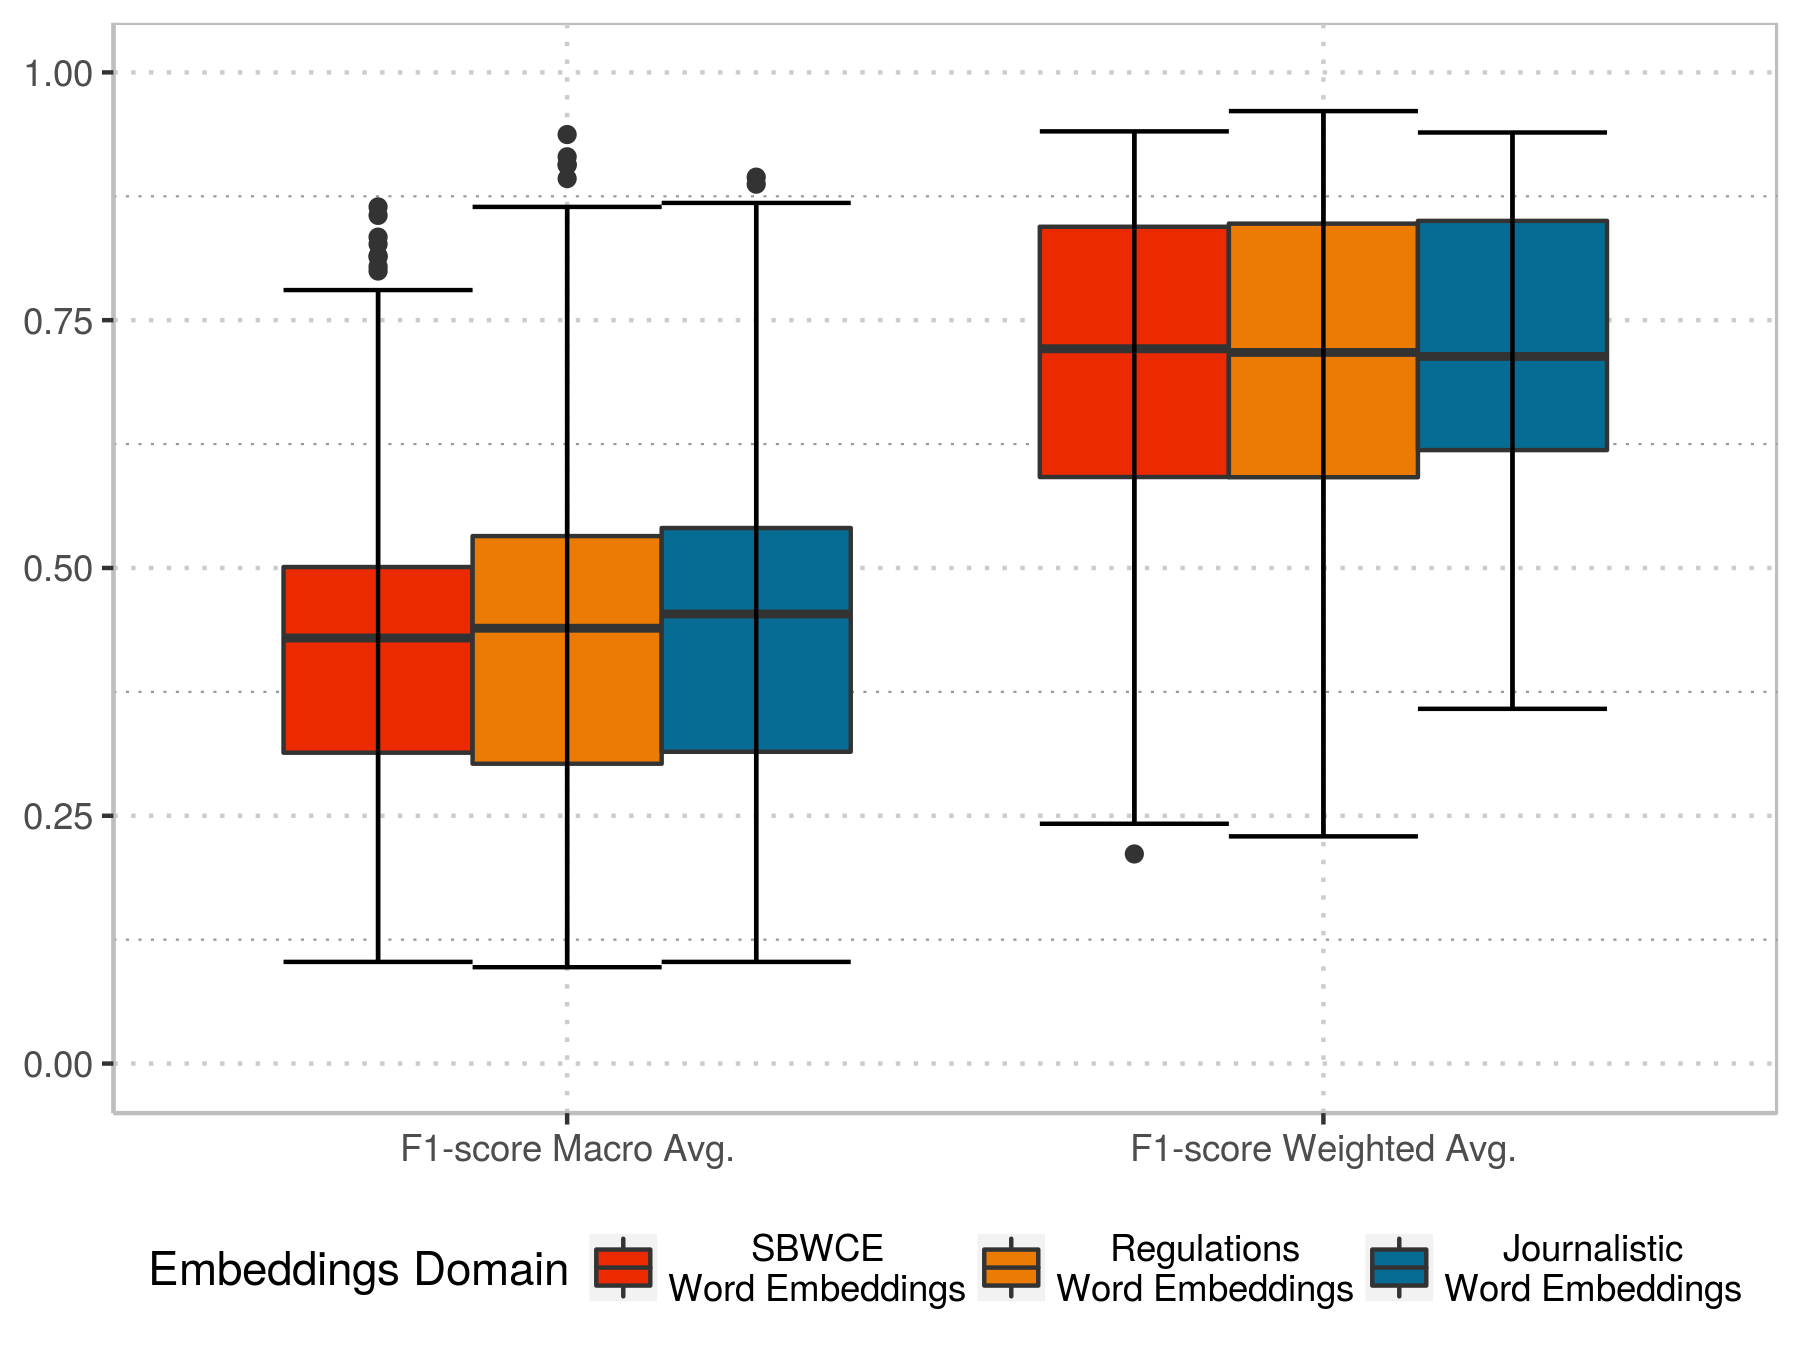
\includegraphics[width=\textwidth]{plots/embeddings/general_vs_out_domain}
  \caption{Performance per lemma on the test corpus for general, specific
  in-domain, and specific out-of-domain embeddings.}
  \label{fig:embeddings:performance_general_out}
\end{figure}

Figure \ref{fig:embeddings:performance_general_out} reports the performance
results on the test corpus for each lemma using these three different domains
to train the word embeddings. The plot is a box and whiskers plot structured in
the following way:

\begin{itemize}
  \item Each group of box-plots shows the different metrics: F1-score macro
    and weighted average.
  \item Each box-plot of a different color shows the performance for
    different training domains of word embeddings: general domain (SBWCE),
    specific domain outside the task (Regulations), and specific domain of the
    task (Journalistic).
  \item The box and whiskers plots represent the distribution of the values of
    the metrics through their quartiles. Each value is the performance for a
    lemma of the corpus. The black thick line in the middle of a box-plot
    represents the median and the whiskers at the end of each box-plot
    represents maximum and minimum value (except for eventual outliers
    represented by black dots outside the box-plot).
\end{itemize}

From the figure, it is noticeable the increase in performance of the median of
the experiments with journalistic, in-domain word embeddings with the F1-score
macro average. Besides the better median, the maximum values are also higher
for in-domain embeddings than for general domain embeddings. In the case of
the F1-score weighted average there is less error  for in-domain embeddings
than for general or out-of-domain embeddings, and the difference for the median
in favor of the general corpus is marginal. Recall that the macro average is
good to measure the performance for the minority classes. Since it is clearly
better for the journalistic in-domain word embeddings, it shows that in-domain
specific word embeddings model less frequent senses better. 

On the other hand it is not clear if the regulations out-of-domain embeddings
affect performance negatively or positively. They show better performance in
some of the better models and worse in some of the worse models, as is
reflected in a wider spread of the whiskers. Thus, I find a clear sign that I
need a close look to each model and see in particular which are the lemmas that
are doing better and which are the ones doing worse. In particular, I need to
look into the outliers. The plot shows that there are 4 (or maybe 5) lemmas
which have better performance with out-of-domain embeddings than with in-domain
embeddings. In any case the journalistic word embeddings are still better in
the general terms for both metrics, because they reduce error.

The reasons behind this results can be many. As a first explanation, the
regulation corpus may not be as dissimilar to the journalistic domain as I
would have expected a priori. A better corpus to test this hypothesis might be
one based in documentation which can be very technical. However, the available
corpus to train such an embedding, at this stage, was not big enough. A line of
future work is to obtain more documentation via web scrapping and train an
embedding from that.

Another possible explanation, which requires the analysis from the point of
view of a linguist expert, is that there are some lemmas (and thus some models)
which show better performance in the particular domain of regulations and thus
this is reflected in the results. This better performance may be due to a
higher frequency in the regulations corpus of words that are relevant to
distinguish senses for that lemma. This line of work will be pursued in future
research.

Finally, the SBWCE has some noise due to the size of the corpus, another line
of future work can be in that area, with embeddings trained from a cleaner
version of the SBWCE.

From these results I have strong evidence to accept the Hypothesis statement,
as the domain from where the word embeddings are trained effectively affects
the final performance of a model.

\subsection{Performance comparison of supervised and semi-supervised
representations}\label{sec:embeddings:results:supvsem}

Hypothesis \ref{hyp:embeddings:2} states that using word embeddings
produces less tendency to overfit over supervised models. Next section reports
the results regarding that hypothesis in order to accept it or reject it.
However, so far I have only compared the results of different word embeddings
for the models.

In this Section, before showing the results of the experiments for Hypothesis
\ref{hyp:embeddings:2}, I want to show how these new models perform in
comparison to the models selected in Chapter \ref{chapter:supervised}. Recall
the final model I want to compare is the multilayer perceptron classifier with
three layers.

Again I follow the steps of Experiment \ref{exp:embeddings:1} that trains a
model with the whole dataset and evaluates such model in a test dataset. For
these results the chosen representations are the hashed hand-crafted features
for the supervised approach and the specific (journalistic) domain word
embeddings for the unsupervised approach.

\begin{figure}[ht]
	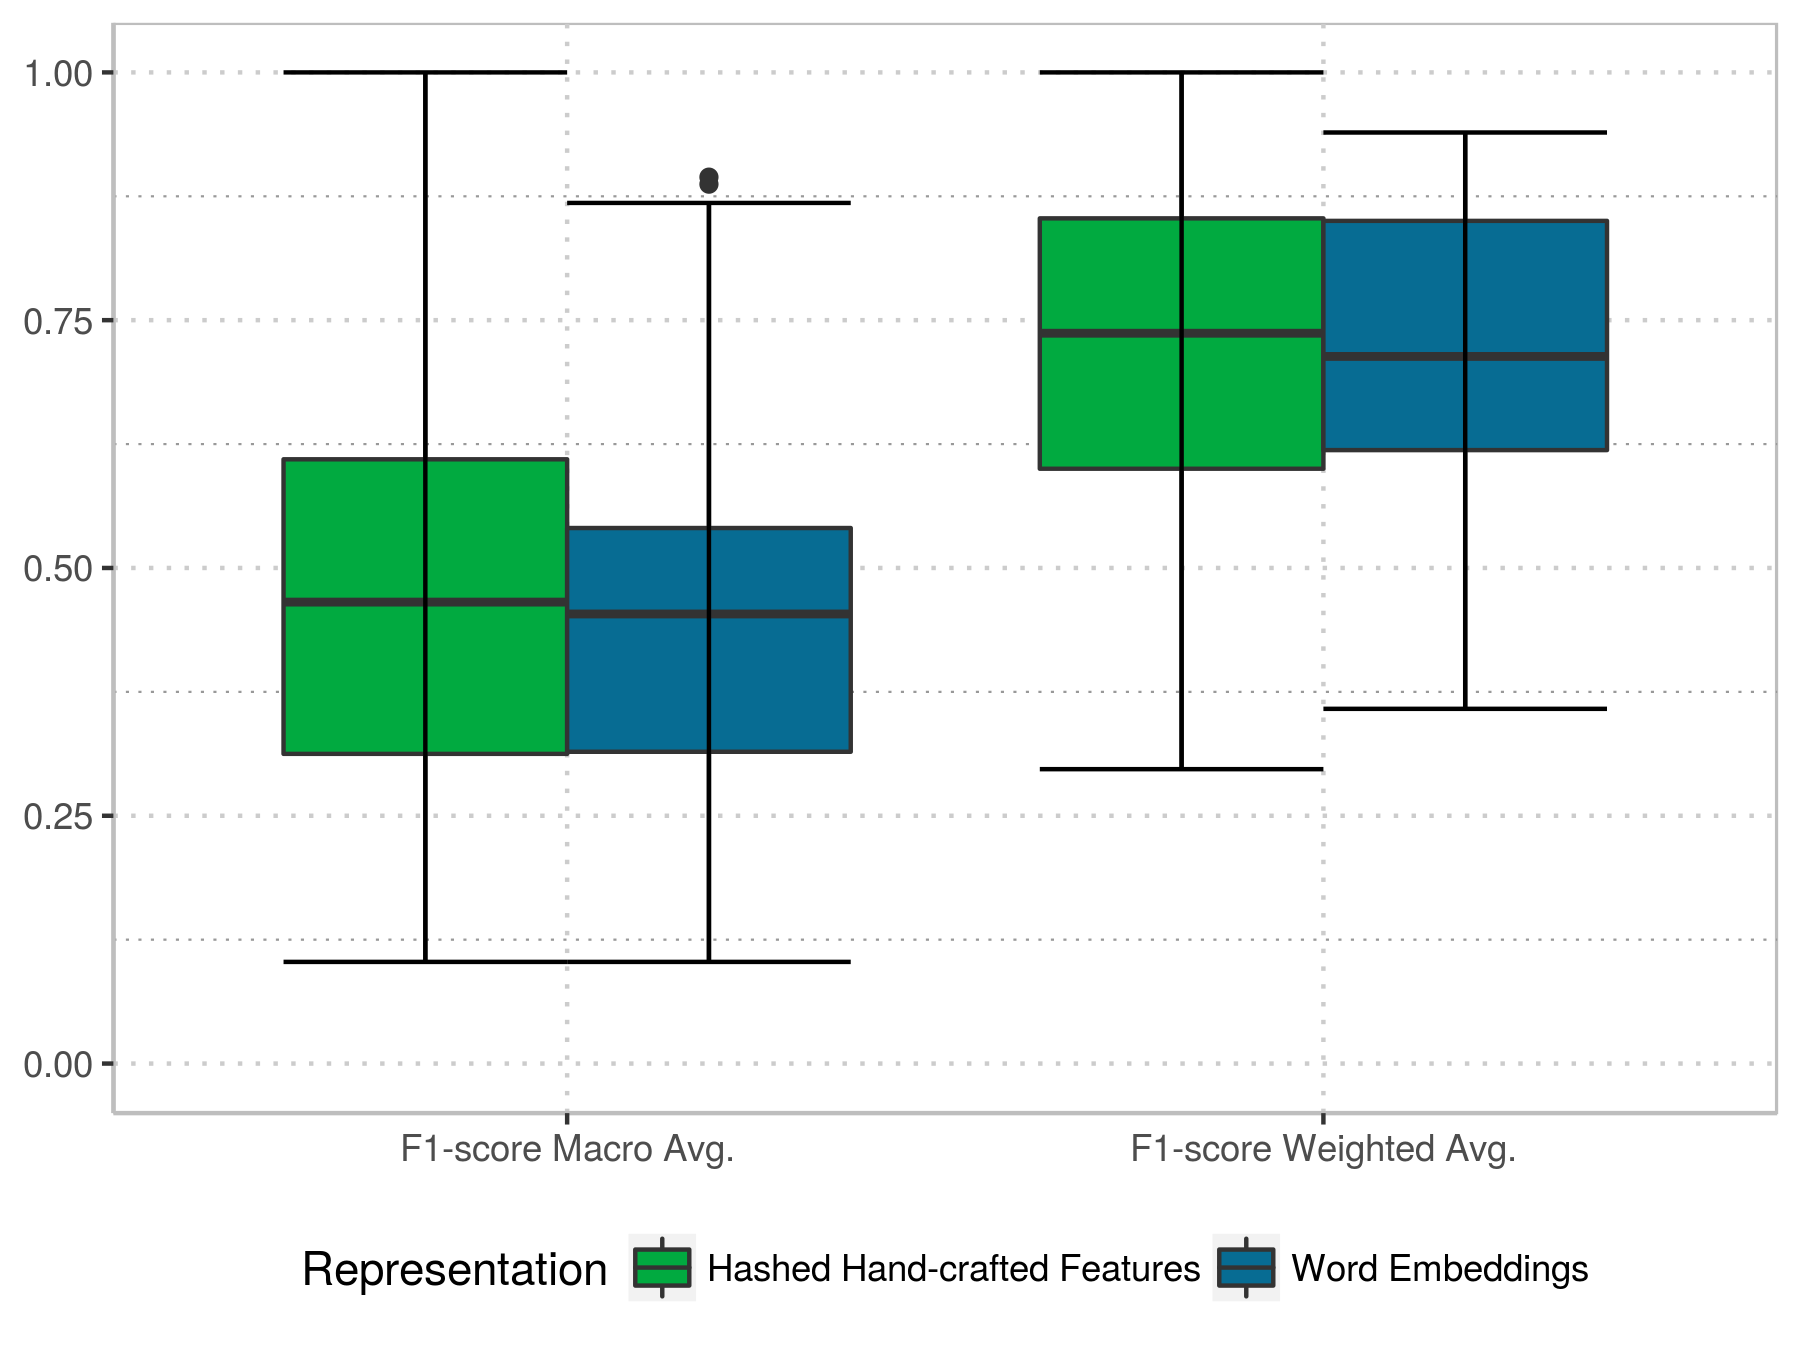
\includegraphics[width=\textwidth]{plots/embeddings/supervised_embeddings}
  \caption{Performance per lemma on the test corpus for hashed hand-crafted
  features and word embeddings of specific domain}
  \label{fig:embeddings:performance_supervised_embeddings}
\end{figure}

Figure \ref{fig:embeddings:performance_supervised_embeddings} reports
the results of Experiment \ref{exp:embeddings:1} and testing it in the held
out test dataset. As in previous Figures, it uses a box and whiskers plot to
display the distribution of the results for each model:

\begin{itemize}
  \item Each group of box-plots shows the different metrics: F1-score macro
    and weighted average.
  \item Each box-plot of a different color shows the performance for different
    representations. For the supervised representation I use the hand-crafted
    hashed features. For the unsupervised representations I use a specific
    domain of the task (Journalistic).
  \item The box and whiskers plots represent the distribution of the values of
    the metrics through their quartiles. The same as explained for Figure
    \ref{fig:embeddings:performance_supervised_embeddings}.
\end{itemize}

In Figure \ref{fig:embeddings:performance_supervised_embeddings} it can
be seen a clear advantage of hashed hand-crafted features over word embeddings.
F1-score macro average performs specially better, indicating that those senses
with low occurrence count are better represented. 

Word embeddings serve as a way of smoothing features by reducing the
dimensionality to a lower, more general representation. Besides, the
representation from which the embeddings are obtained takes into account less
features than hand-crafted features. Indeed, hand-crafted features encode
syntactic and PoS information, while to obtain word embeddings only word
co-occurrences are used.

Taking this into account, it can be interpreted that hand-crafted features
represent the domain better than the semi-supervised model. This may be due to
the fact that the features are taken from the supervised data itself, unlike
the journalistic word embeddings, which are taken from a corpus that shares
domain with the supervised data. Supervised features have a better performance
because they can fit more closely to the data, and that is the reason why
supervised features are less able to generalize a model, specially a domain
driven model, into data from more general domain. In the next section I will
explore the tendency of these models to overfit or generalize.

The adequacy of these two kinds of models to adapt to an out-of-domain corpus
will be displayed in the following Chapter. There we will see that word
embeddings are able to perform well on a self-learning approach on a big
corpus. In contrast, hand-crafted features fail to generalize and their
performance quickly degrades across iterations.

\subsection{Hypothesis \ref{hyp:embeddings:2}}\label{sec:embeddings:hyp:2}

The results of the previous section showed that supervised features perform
better than unsupervised features for the \vsd~task. The results of the
experiments for Hypothesis \ref{hyp:embeddings:2} give a hint on what is
happening underneath these results.

These results are taken from Experiment \ref{exp:embeddings:2}, and report the
learning curve of a model as the number of examples increases. It shows the
mean and error due to variance of both the training and test sets on each
iteration. The comparison is done using a supervised representation via hashed
hand-crafted features and an unsupervised representation via word embeddings,
in this case the specific domain word embeddings.

\begin{figure}[ht]
	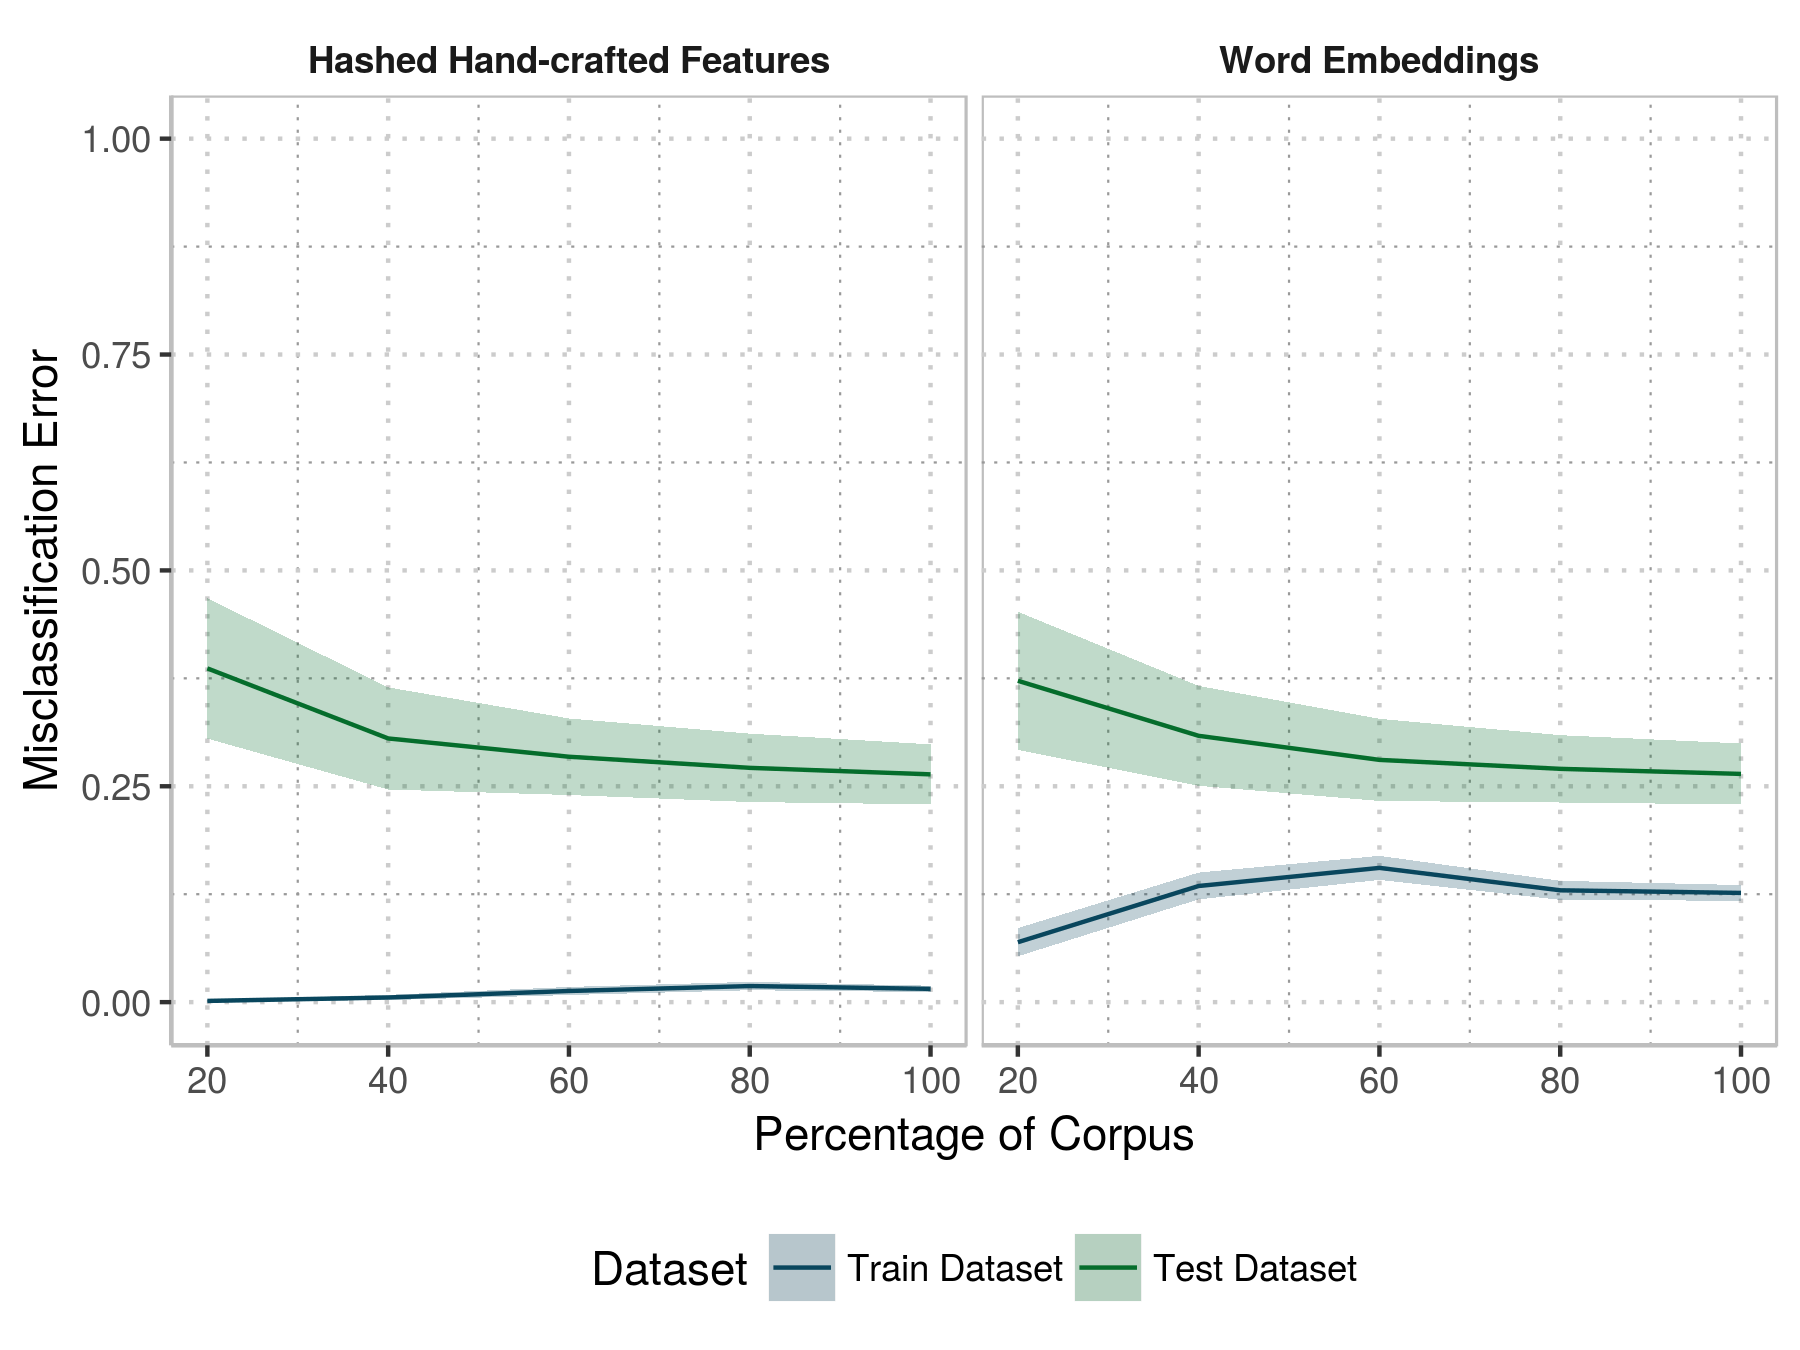
\includegraphics[width=\textwidth]{plots/embeddings/learning_curve_scores}
  \caption{Learning curve for different sizes of training corpus for supervised
  and unsupervised representations}
  \label{fig:embeddings:learning_curve}
\end{figure}

Figure \ref{fig:embeddings:learning_curve} shows the learning curve for
different sizes of the training data over two different representations for the
input features: supervised hand-crafted features and unsupervised word
embeddings. The structure of the learning curve plot is as follows:

\begin{itemize}
  \item The plot is divided in two columns, each represents an input to the
    model: supervised hand-crafted features and unsupervised word embeddings of
    the specific domain (journalistic).
  \item The x-coordinate shows the size of the training data, as a percentage
    of the total training data available, starting from 20\% of the corpus (the
    corpus was split in 5 parts according to Experiment
    \ref{exp:embeddings:2}).
  \item The y-coordinate shows the misclassification error of a model.
  \item There are two colors representing the datasets: train and test.
  \item The solid darker lines represent the mean of misclassification error
    trough the different splits of the datasets over all the models.
  \item The shadowed area, which has a lighter color, represent the standard
    error of the mean of the misclassification error.
\end{itemize}

It is possible to see in the Figure the difference between representations when
the tendency to overfit is measured. Word embeddings show less difference
between the training data and the test data regarding misclassification. This
could also be seen in Section \ref{sec:supervised:hyp:4}, where SVM and Naive
Bayes showed less tendency to overfit the model.

In this case the classifier is a non linear classifier with a strong tendency
to overfit, and the word embeddings are helping it to not overfit as much as
the supervised representation does. Still, it is important to note that the
misclassification error in test data is still roughly the same for one
representation or the other, thus the model is not sacrificing training
performance in order to gain test performance. What the model is actually
sacrificing is anecdotal, non-generalizing information. These results support
evidence to accept Hypothesis \ref{hyp:embeddings:2}. 

It is important to recall that the models are small and neural networks models
work better the more information they have. In order to gather more
information, more examples are needed. However, manual annotation of examples
is expensive and beyond my possibilities. Thus I pursue increasing the number
of examples available to the model via incorporating examples from unsupervised
corpora. And to do so we need models which generalize better to out-of-domain
corpora, as is the case of models with word embeddings. 

\section{Conclusions}\label{sec:embeddings:conclusions}

This chapter introduced a disjoint semi-supervised technique for Spanish \vsd.
From the challenges stated in Chapter \ref{chapter:supervised} I wanted to
overcome the shortcoming of having a model with a high tendency to overfit the
data. I stated a main hypothesis I want to test, which is that unsupervised
representations help improve upon purely supervised models by reducing the
tendency to overfit given by features taken from the same data where the model
is trained. The reason to state this hypothesis is that unsupervised
representations give a smoothed version as input to a classifier and thus this
helps the classifier in having a more generalized version of the data it is
learning from. I subdivided the hypothesis in smaller, more focused
subhypotheses.

Hypothesis \ref{hyp:embeddings:1} states that the performance of an
unsupervised representation, in this case a word embedding, depends on the
domain from where the unlabeled data to train the embeddings is taken. The
results to accept this hypothesis are in Section
\ref{sec:embeddings:hyp:1}. It was shown that a more specific domain gives
better results for the same task. Still some of the results regarding the use
of a domain outside the domain of the supervised need a more thorough analysis
left for future work.

Before analyzing the results of the experiments to test Hypothesis
\ref{hyp:embeddings:2} I needed a comparison between supervised and
unsupervised representations. This is reported in Section
\ref{sec:embeddings:results:supvsem}. In this experiment I train two
different models using the neural network classifier with three layers
described in Section \ref{sec:embeddings:classifiers}, and changing the
input representation for the classifier. From this comparison, hand-crafted
features show better performance than the unsupervised features. However the
reason behind this is that hand-crafted features obtain a more fitted
representation  of the supervised dataset as the features come directly from
there. The results of the experiments to test Hypothesis
\ref{hyp:embeddings:2} show that hand-crafted features are strongly
dependent on the dataset, and that the resulting representation is highly
fitted to the training examples.

Section \ref{sec:embeddings:hyp:2} shows the results of Experiment
\ref{exp:embeddings:2}, which measures the tendency to overfit of a
classifier. The experiment is done to test Hypothesis
\ref{hyp:embeddings:2}, which states that unsupervised representations
(e.g. word embeddings) produce less overfitting over the supervised models than
supervised representations (e.g. hand-crafted features). The experiment
compared hashed hand-crafted features and specific domain word embeddings. As
the hypothesis states, the model trained with word embeddings showed a closer
learning curve between training and test data. This gives enough evidence to
support the acceptance of Hypothesis \ref{hyp:embeddings:2}.

Unsupervised feature representations, particularly those trained from the same
domain as the supervised dataset, show promising results. However, the
performance is still under what I can achieve using purely supervised
representations. And although there can be many reasons to explain this result,
according to what I see, most likely it has to do with the (over)fitting of the
supervised features to the supervised data, in contrast to the more smooth
representation of word embeddings.

Recall from the previous Chapter I found two main challenges. The first
challenge was that models trained with little data tend to overfit. Using
non-linear classifiers such as neural networks could have a great impact in
minimizing the error and even maximizing the performance of the test data. But
the cost is the generalization of such models. Unsupervised features help in
that respect by giving a smoother representation helping the neural network to
avoid the tendency to overfit.

The other challenge was the coverage of the model. Coverage can be understood
as the ability to predict over unseen examples that belong to one of the target
classes and the model should be able to label. These examples could eventually
be incorporated to the training corpus and thus add information to the model.
But since they are not annotated, the model does not have such information yet.
Given our limitations to annotate examples manually, new examples are gathered
from unlabeled data and classified with the model. If the model is only driven
by the information it already has (i.e. the features extracted from the
supervised data), then is difficult to add the information from unseen data and
expand the coverage. Word embeddings hold information about the supervised
data, used for the model to classify it, and about unsupervised data not
present in the model yet. Thus, this information helps a model trained from
unsupervised features generalize better and be able to gather information from
new examples expanding its coverage.

Following these reasons, word embeddings seem specially adequate to apply an
approach to obtain new examples from previously unseen corpus.

In the next chapter I will focus on a first approach to a semi-supervised
method which adds data from unlabeled sources and use that to expand the model.
Such method is self-learning, a basic approach to semi-supervised learning.

Future work of this chapter includes using other unsupervised representations,
like the ones listed by Turian et al. \cite{Turian:2010:WRS:1858681.1858721}:
Collobert and Weston \cite{Collobert:2008:UAN:1390156.1390177} and Brown
clusters \cite{Brown:1992:CNG:176313.176316}. Another line of work would be
doing a more thorough error analysis on the the different word embeddings
domain, seeing if a better preprocessing of the data can provide better
results. 
